\documentclass{article}
\usepackage[french]{babel}
\usepackage{../faustin}
\usepackage{minted}

\definecolor{bg}{rgb}{0.85,0.85,0.85}
\newenvironment{sql}{%
\VerbatimEnvironment
\begin{minted}[linenos, bgcolor=bg,numbersep=5pt,framerule=1pt,frame=lines,numberblanklines=false,fontsize=\footnotesize]{sql}%
}{%
\end{minted}
}

\definecolor{ups}{HTML}{63003C}
\begin{document}
% ----------------------------------------------------------------
\begin{titlepage}
\newgeometry{left=7.5cm} %defines the geometry for the titlepage
\pagecolor{ups}
\noindent
\includegraphics[width=3cm]{../logo.png}\\[-1em]
\color{white}
\makebox[0pt][l]{\rule{1.3\textwidth}{1pt}}
\par
\noindent
\textbf{\textsf{Faustin MILLET}}, élève en 1A
\vfill
\noindent
{\huge \textsf{Projet S104 - Rapport final}}
\vskip\baselineskip
\noindent
\textsf{Janvier 2022}
\end{titlepage}
\restoregeometry % restores the geometry
\nopagecolor% Use this to restore the color pages to white
% ----------------------------------------------------------------
\pagestyle{fancy}
\fancyhf{}
\lhead{Faustin MILLET}
\chead{Projet S104 - Rapport final}
\rhead{\today}
\fancyfoot[R]{Page \thepage/\pageref{LastPage}}
{
\hypersetup{linkcolor=black}
\tableofcontents
}

{\color{ups}
\vspace{24pt}
\hrule
\vspace{12pt}
Malgré mes relances sur son adresse email personnel, Daniel m'a laissé seul sur ce projet. Ses absences aux séances de projets, m'ont empéchés de pouvoir travailler en groupe avec lui. \textbf{Devant réaliser l'intégralité du travail moi-même, je vous prie de bien vouloir adapter la correction à cette situation.}
\vspace{12pt}
\hrule
\vspace{12pt}}

\newpage

\part{Présentation de l'entreprise}
\setcounter{section}{0}
\href{https://foodymix.fr/}{Foodymix} est une startup qui livre des paniers recettes à des particuliers. Les clients font une sélection de recettes et reçoivent les ingrédients associés à ces recettes pour ensuite les cuisiner avec un robot cuiseur. Elle met en relation des fournisseurs dans son secteur géographique et des clients partout en France à l'aide du prestataire \href{https://www.chronofresh.fr/fr}{Chronofresh}. L'entreprise est située à Avignon et travaille donc principalement avec des fournisseurs dans un secteur proche.
La startup est inscrite dans la démarche French Tech. Elle cherche donc à innover et se développer en réseau avec d'autres entreprises.

L'entreprise a été crée il y a un an, mais sa commercialisation n'a eu lieu qu'il y a 6 mois. Sur le plan légal, l'entreprise a été crée par deux associés, deux frères, en tant que SAS. L'objectif était de pouvoir vendre des parts et obtenir du capital plus facilement.

Malgré sa jeunesse, l'entreprise est en pleine croissance et doit adapter ses différents process à sa popularité. L'entreprise possède trois salariés, les deux cofondateurs qui ne se versent pas de salaire et une alternante.
\begin{figure}[h]
    \centering
    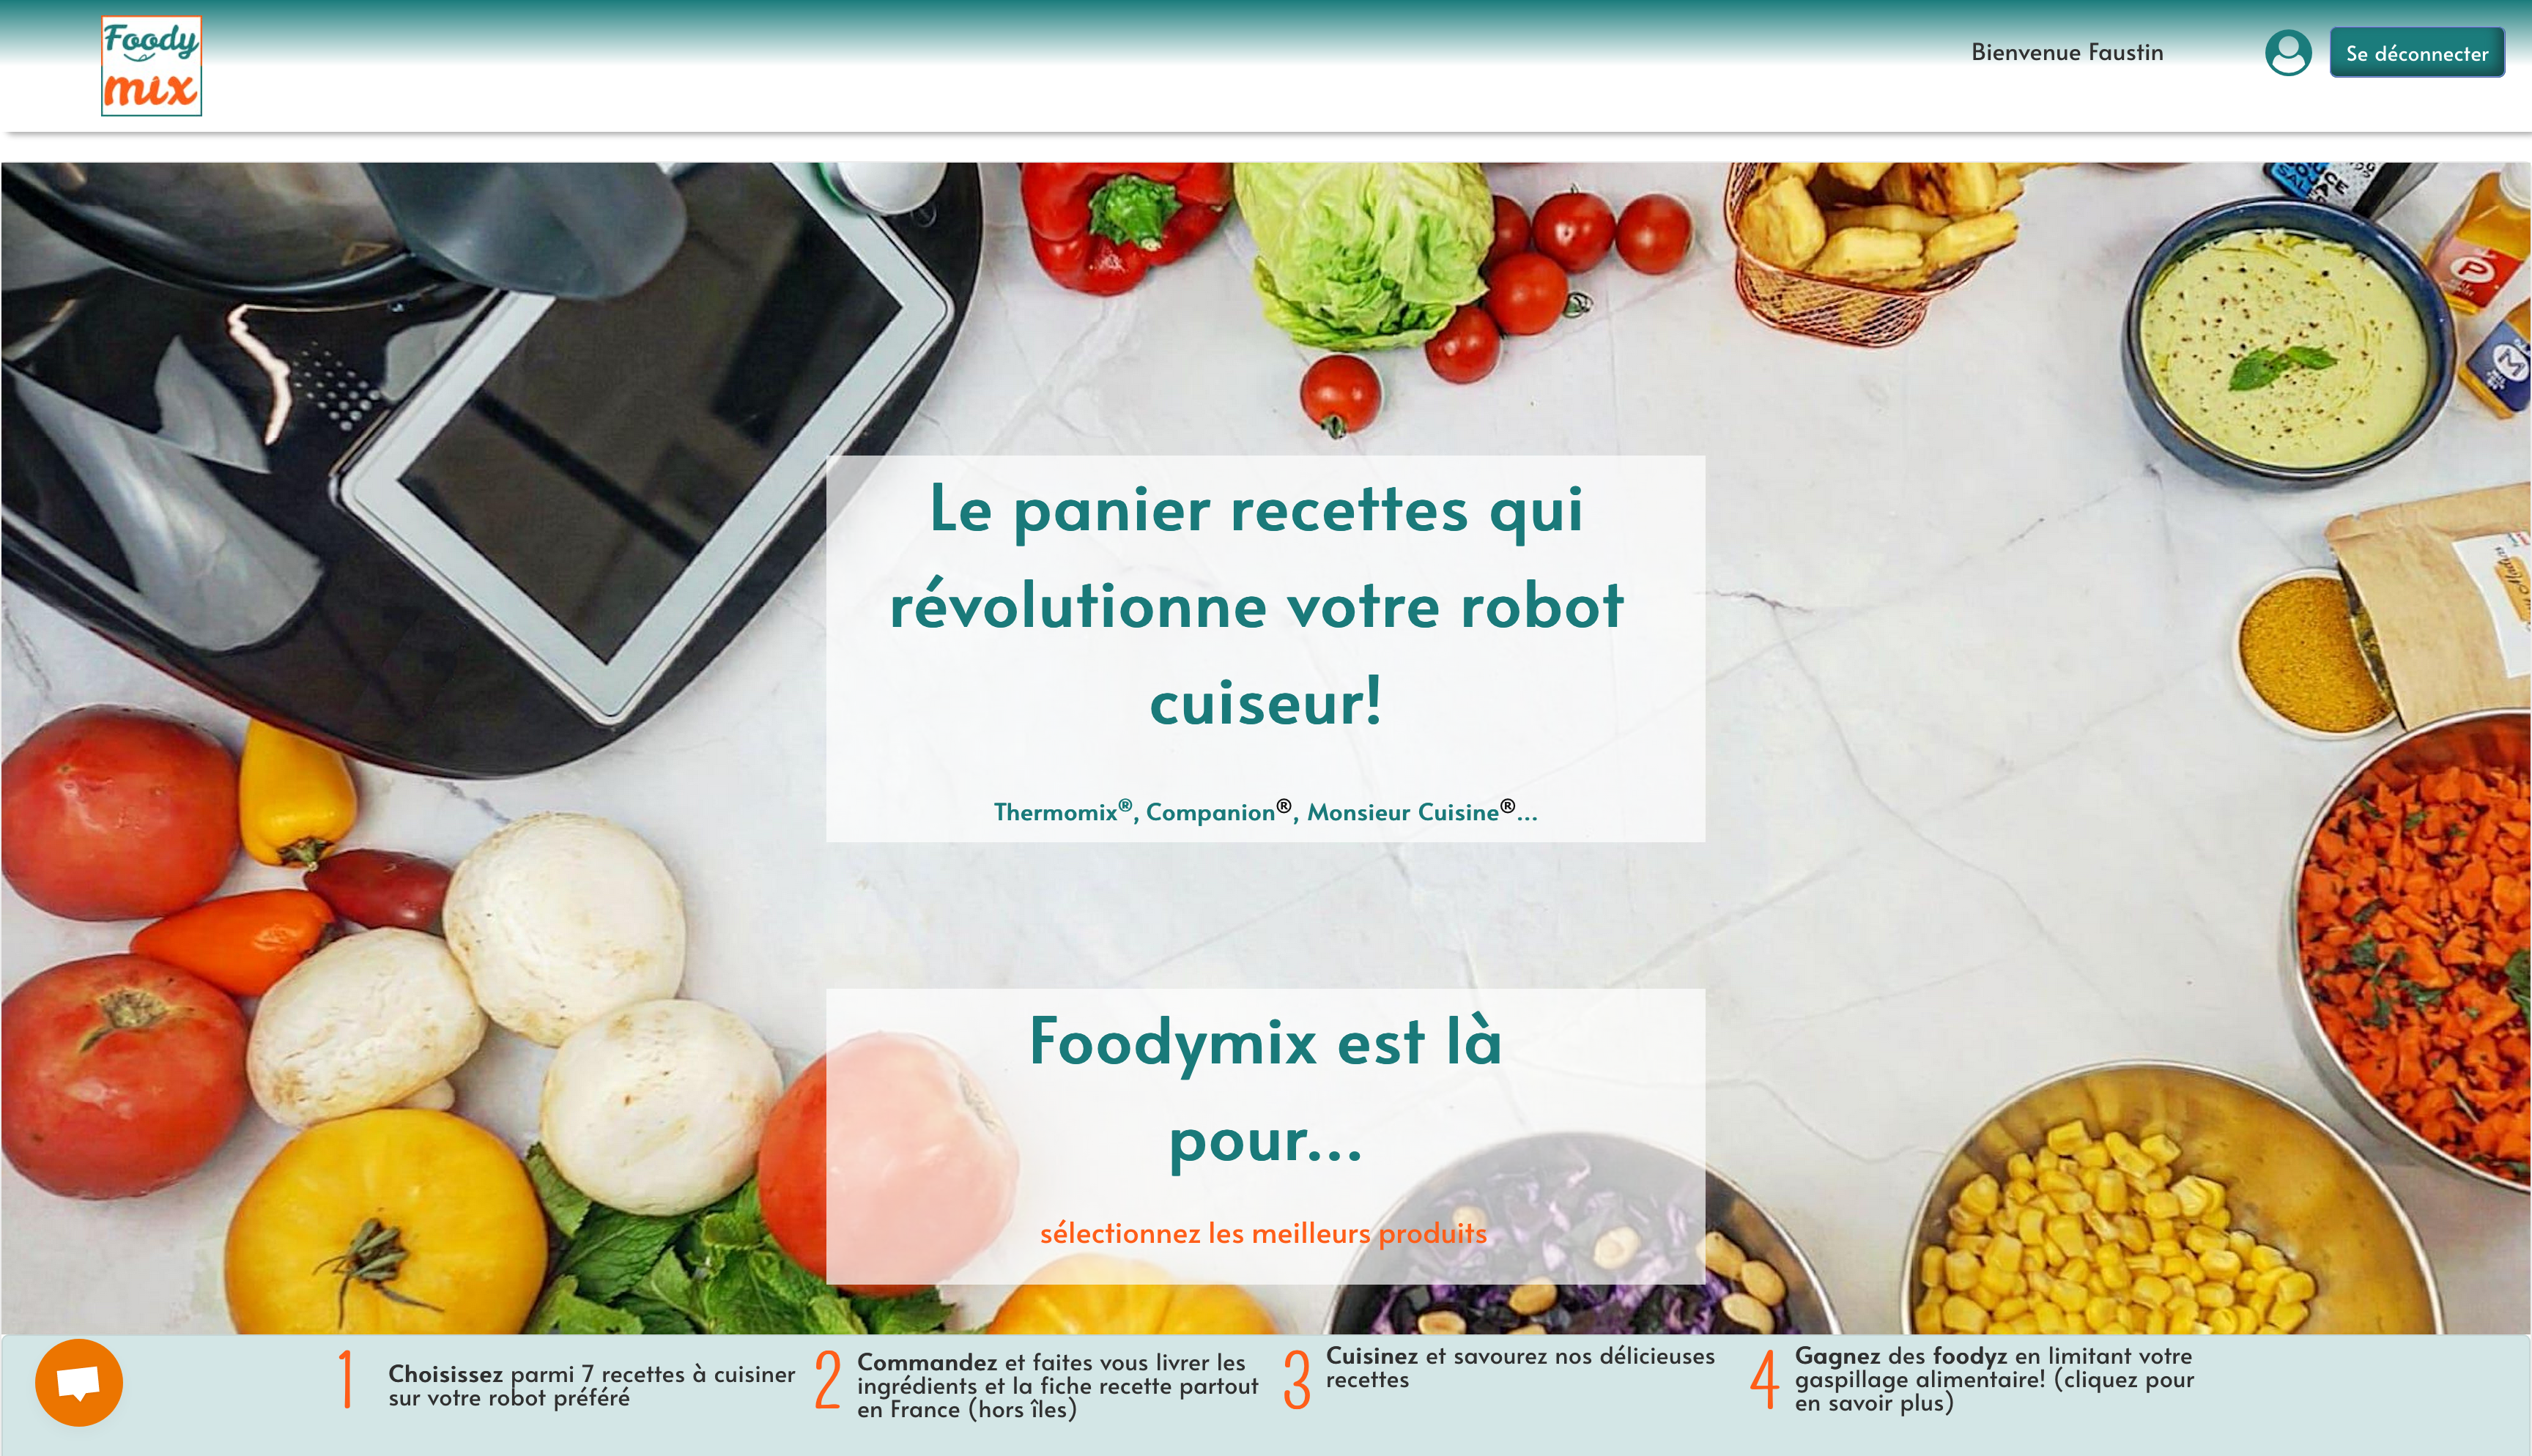
\includegraphics[width=0.8\linewidth]{images/foodymix.png}
    \caption{Page d'accueil du site de \href{https://foodymix.fr/}{Foodymix}, le jeudi 3 novembre}
\end{figure}
\section{Mise en relation}
À l'aide d'une relation familiale, j'ai pris contact avec Anthony Poirier, cofondateur de la startup. M.Poirier est chargé des systèmes d'informations, principalement le site boutique, et de la coordination du marketing. J'ai présenté mon projet universitaire par mail et Anthony Poirier été ravis de participer à ce projet. Nous avons donc convenu d'un entretien téléphonique vendredi 21 octobre.

Nous avons eu un entretien téléphonique d'une heure, au cours duquel nous avons discuté de l'entreprise, de ses besoins et de sa gestion des données.

En amont de cet entretien, j'avais navigué sur le site web pour lister les différentes données utilisées. Par exemple, la page d'inscription ou une page recette. M.Poirier m'a confirmé au téléphone, les observations que j'avais faites et il m'a également fourni des détails sur le fonctionnement de l'entreprise vis-à-vis de ses fournisseurs et certaines spécificités sur la logistique.

\part{Besoins de l'entreprise}
\setcounter{section}{0}
L'entreprise a donc des spécificités propres à son activité. Tout d'abord, il y a une partie commune à toutes les boutiques en ligne. Ensuite une partie spécifique à l'activité de Foodymix, la logistique alimentaire. Enfin, une relation à entretenir à la fois avec ses clients et ses fournisseurs.
\section{Gérer des recettes}
Tout d'abord Foodymix contient plusieurs recettes. Les recettes de cuisine contiennent plusieurs ingrédients, ont une durée fixe ainsi qu'un titre et une description.
L'organisation est très similaire à un site comme Marmiton, à l'exception de la partie communautaire.

\begin{figure}[h]
    \centering
    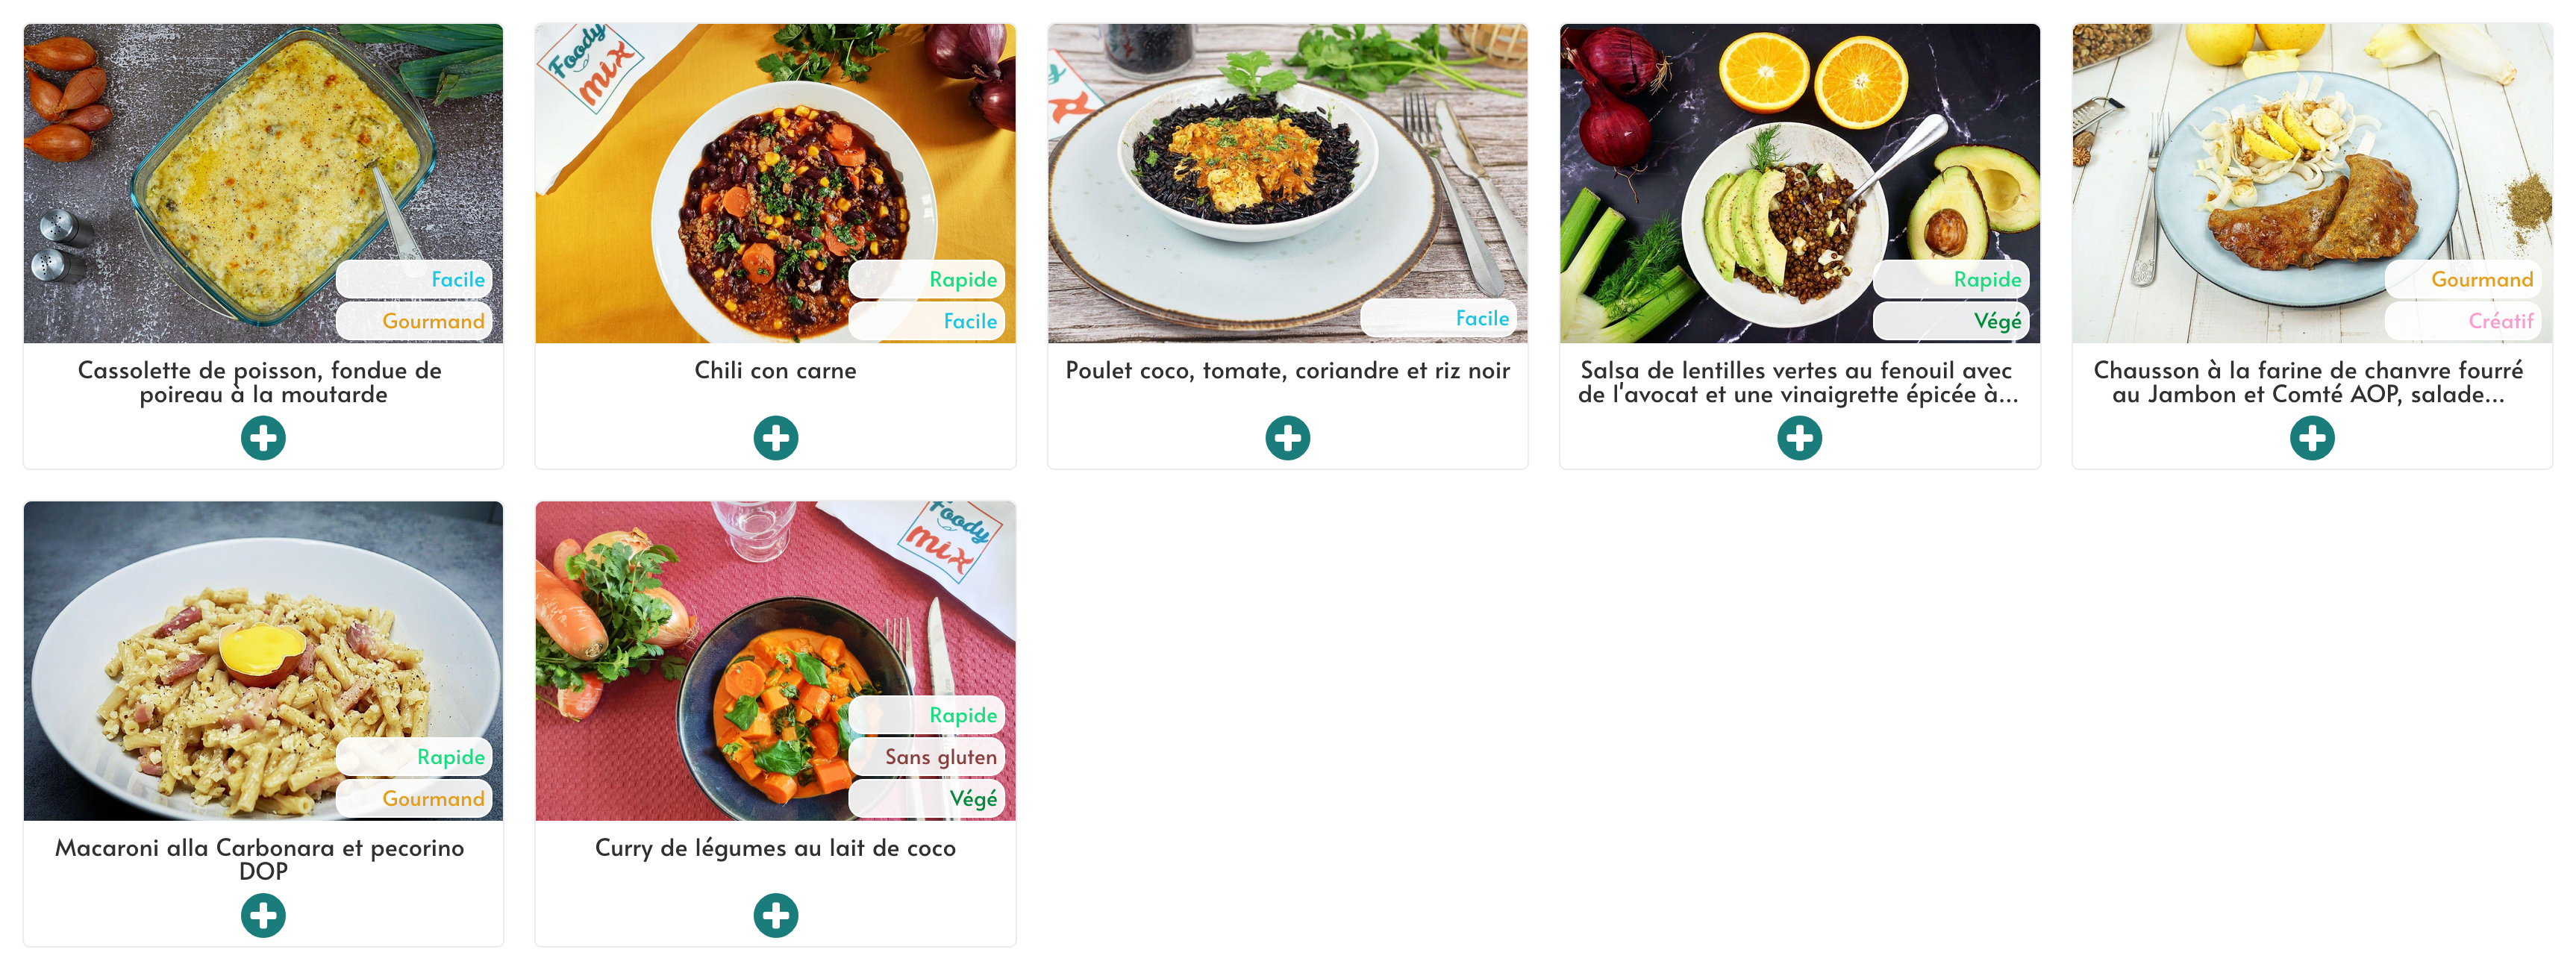
\includegraphics[width=0.8\linewidth]{images/recettes_foodymix.png}
    \caption{Liste des recettes du site de \href{https://foodymix.fr/}{Foodymix}, le jeudi 3 novembre}
\end{figure}

Foodymix propose des recettes différentes chaque semaine. Les recettes sont choisies suivant la saisonnalité et la disponibilité des produits, la diversité avec les autres recettes de la semaine et enfin la nouveauté des recettes. Le process de sélection est géré par l'équipe du site.

Les recettes sont labellisées principalement pour que le client découvre en un clin d'œil si la recette correspond à ses goûts. Sachant que l'entreprise souhaite dans le futur proposer des recettes personnalisées en fonctions des goûts des clients

\begin{figure}[p]
    \centering
    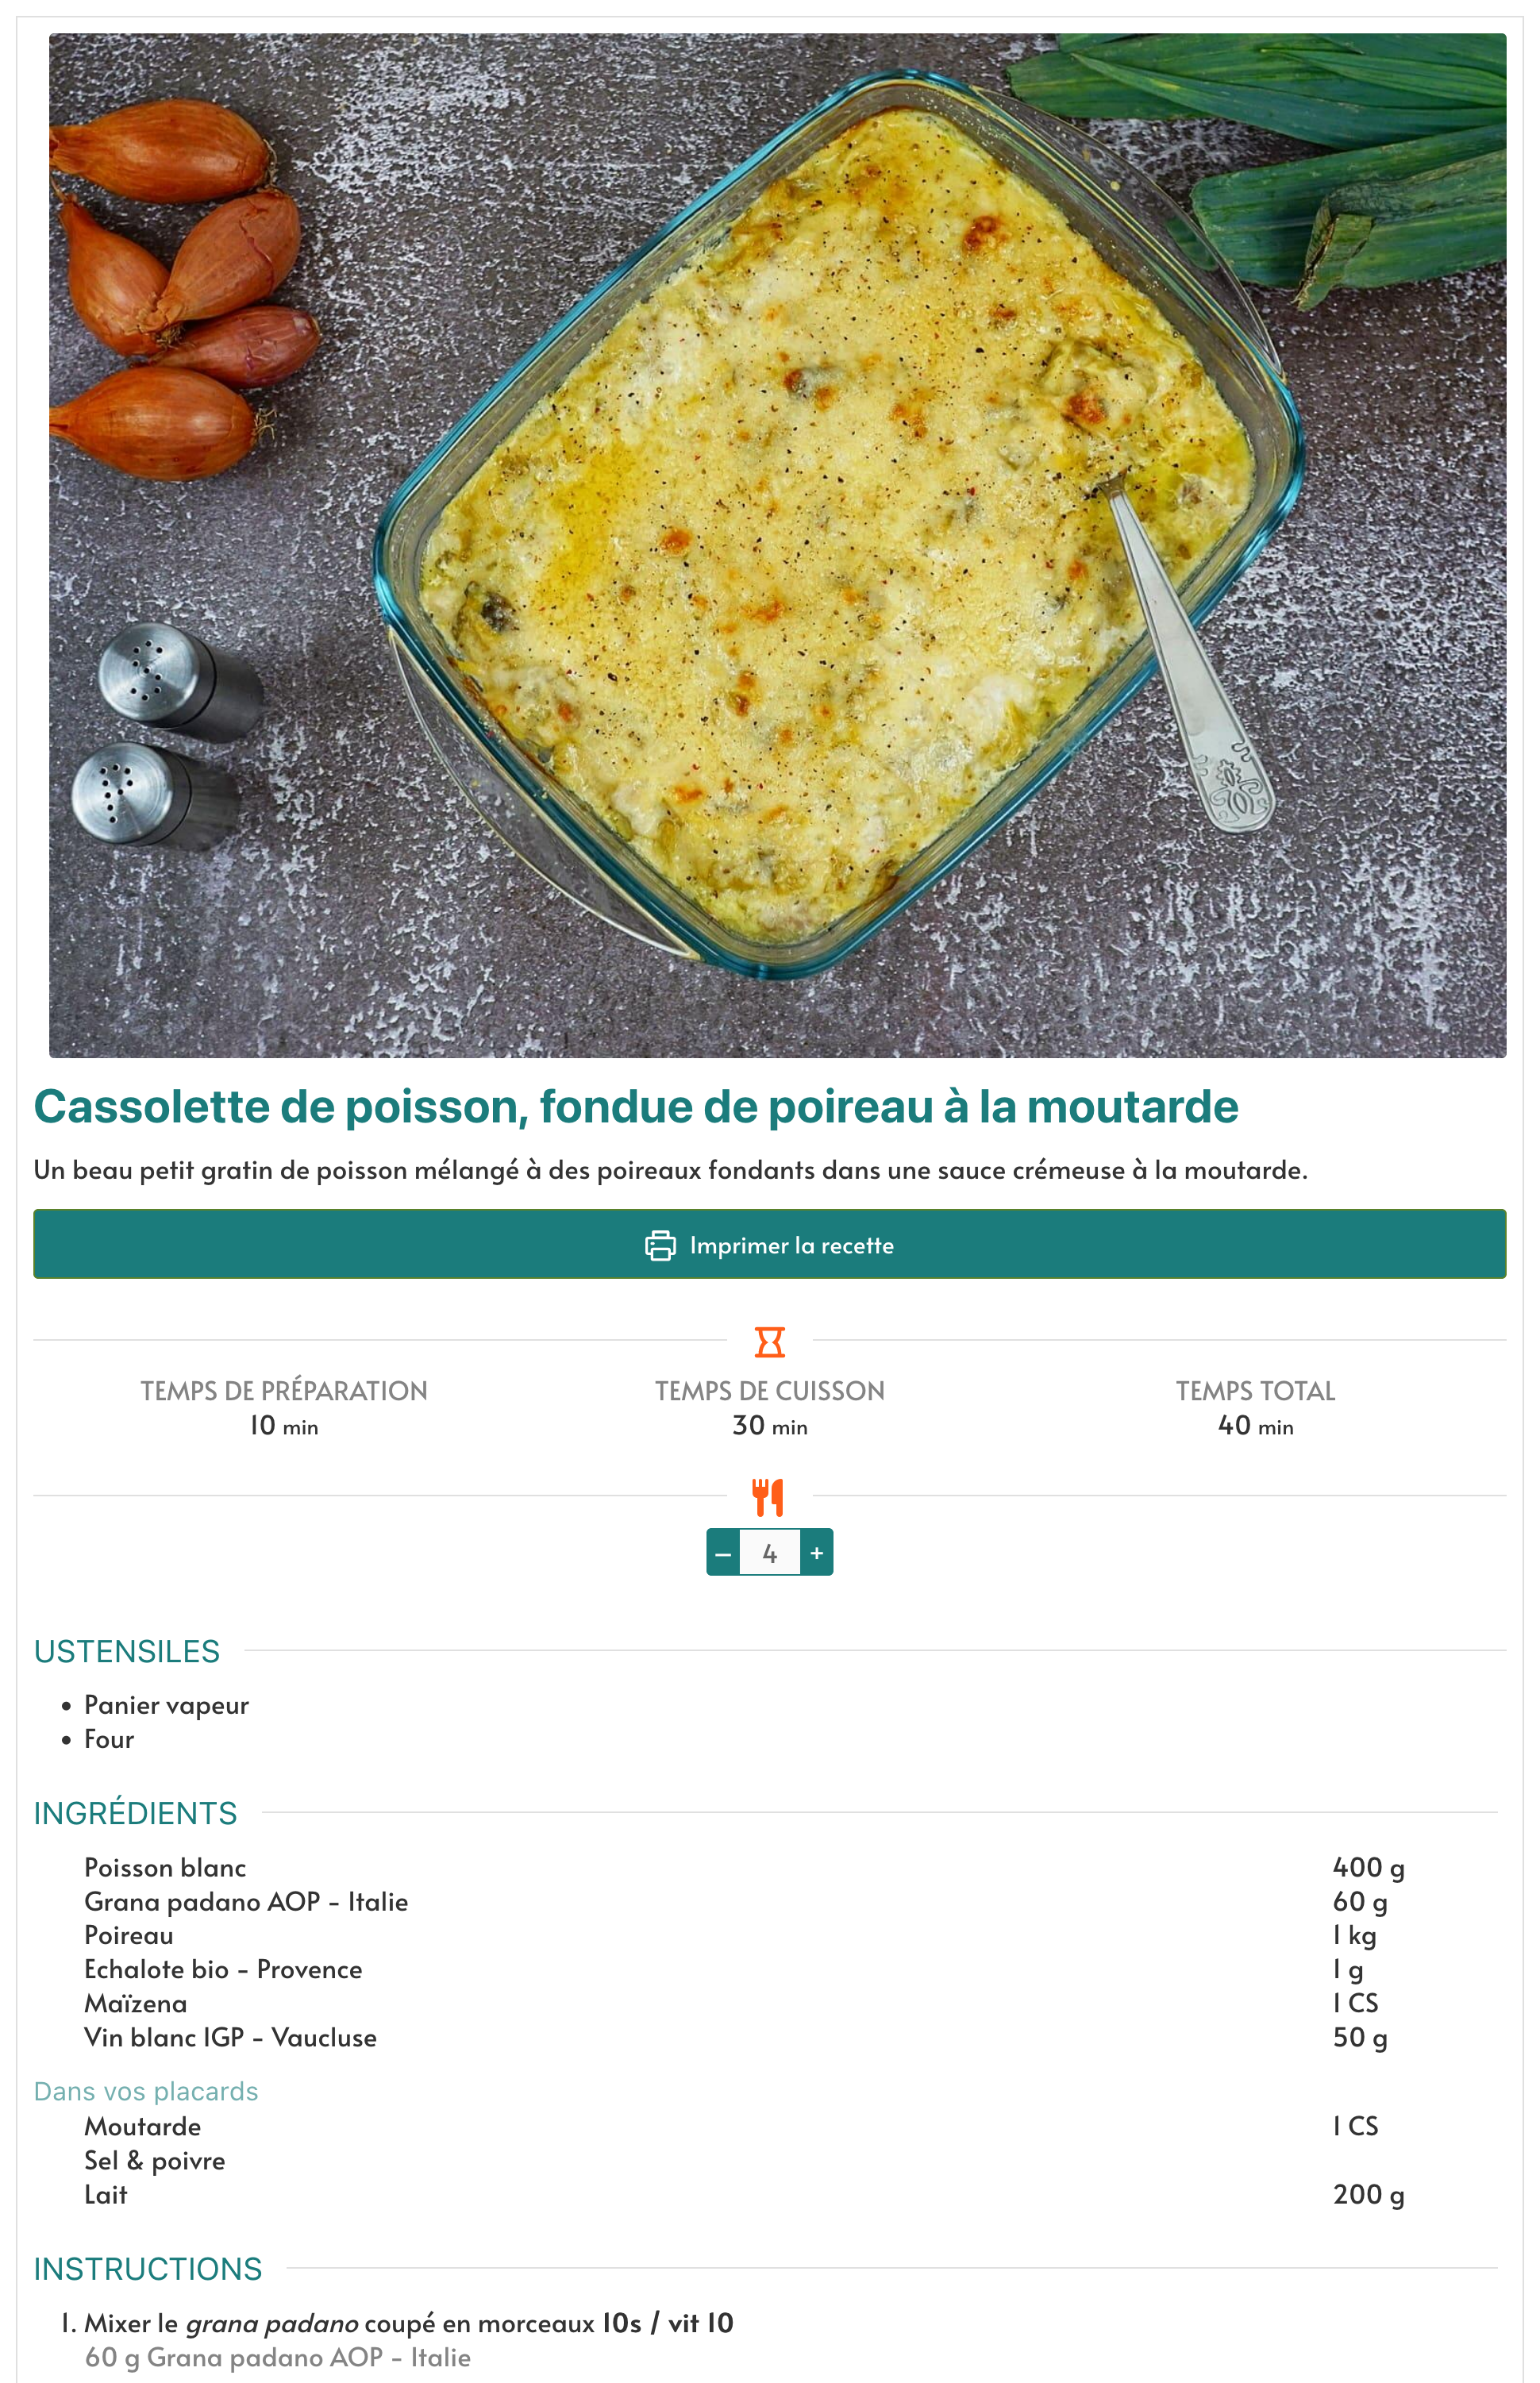
\includegraphics[width=0.8\linewidth]{images/recette_foodymix.png}
    \caption{Exemple de la recette \textit{Cassolette de poisson, fondue de poireau à la moutarde}}
    \label{Figure Recette Exemple}
\end{figure}

\subsection{Les ingrédients}
Gérer des recettes, implique également gérer des ingrédients, ces ingrédients sont indiqués dans les recettes avec leur quantité, l'unité et également leur présence dans le colis. Par exemple, le sel ne sera pas fourni par Foodymix (voir page \nameref{Figure Recette Exemple}). Les recettes sont vendues à la portion, si vous cuisinez pour 4 personnes, vous achèterez donc 4 portions. 

Les quantités pour chaque ingrédient sont pour chaque portion. Or il est simple de conditionner 200 g de farine, mais il est beaucoup plus dur de conditionner 200 g de poisson. L'équipe sait donc si le produit sera conditionné \textit{en vrac} ou à la portion.

Foodymix fait également la distinction du frais dans ses ingrédients pour mieux traiter la logistique, par exemple un produit comme du beurre ne peut être conservé dans un entrepôt et nécessite une non-rupture de la chaîne du froid.
\section{Gérer un e-commerce}
Avant d'être un gestionnaire de contenu, Foodymix est un e-commerce. Chaque utilisateur peut acheter un ou plusieurs repas, dans des quantités variés. Il doit être récompensé et incité à revenir sur le site.

\subsection{Les données personnelles}
La valeur la plus précieuse pour une boutique virtuelle ou physique est sa base client. Elle permet à l'enseigne d'améliorer et de faire grandir son activité tout en fidélisant une clientèle.

\begin{figure}[p]
    \centering
    \includegraphics[width=0.8\linewidth]{images/email_foodymix.png}
    \caption{Newsletter du Lundi 31 Octobre}
    \label{Figure Newsletter}
\end{figure}
Lors de la création d'un compte client, l'utilisateur doit donc rentrer plusieurs informations, nom, prénom, email, numéro de téléphone, etc. Ces informations permettront à l'entreprise de livrer le client, mais aussi de garder le lien avec lui en envoyant des mails régulièrement (voir \nameref{Figure Newsletter}). La gestion de la newsletter est délégué à l'entreprise \href{https://fr.sendinblue.com}{Sendinblue}.
\pagebreak

\subsection{Livraison et facturation d'un client}
Le client inscrit également une ou plusieurs adresses postales pour se faire facturer et indiquer où livrer son colis. L'entreprise propose à chaque client d'inscrire une ou plusieurs adresses. Cependant, un client ne peut avoir qu'une adresse de facturation à la fois, et il ne peut livrer un colis qu'à une des adresses enregistrées sur son compte.
\begin{figure}[h]
    \centering
    \includegraphics[width=0.8\linewidth]{images/adresse_foodymix.png}
    \caption{Gestion des adresses sur le site de Foodymix}
\end{figure}

La livraison de produit frais est une logistique difficile, mais Chronofresh garantie une date de livraison à Foodymix. Cependant d'expérience, Foodymix sait que Chronofresh sera plus long dans certains codes postaux principalement des villes de Bretagne. Il est donc important de vérifier si le client se fait livrer à une de ses villes pour l'avertir des délais.

\subsection{Les clients ambassadeurs}
\label{Sub Ambassadeur}
Certains clients peuvent demander à être ambassadeur de la marque. Ça peut être des vendeurs à domicile de robots ou des influenceurs par exemple. Foodymix va proposer à ces clients un menu supplémentaire dans leur espace personnel, ce menu permettra d'avoir un code promotion qui reverse une commission à l'ambassadeur. Le code promotion est donc unique pour chacun des ambassadeurs.

\subsection{Facturation des clients}
Pour le paiement d'une commande, l'entreprise fait appel à un prestataire : \href{https://paygreeen.io}{Paygreen}. En effet, la loi impose l'utilisation de standards de sécurités très exigeantes et il est rare de voir une petite entreprise gérer elle-même son infrastructure de paiement. Foodymix n'a donc pas accès aux données bancaires de ses clients.

Quand Paygreen indique à Foodymix que le paiement a été effectué, Foodymix édite une facture avec un numéro, la date et les différentes recettes commandées avec le nombre de portions pour chacune.

\subsection{Foodyz}
Foodymix souhaite mettre en avant la lutte contre le gaspillage alimentaire. En commandant sur Foodymix, les quantités sont pensées pour donner pile la bonne quantité. Pour récompenser et fidéliser ses clients, la société donne 41 Foodyz par portion.

Les Foodyz peuvent être échangé contre une récompense. Par exemple, si un client a 2500 Foodyz, il obtient une bouteille d'huile d'olive et 10 € en bon d'achat.

\section{Gérer des fournisseurs}
\subsection{Le circuit court}
\label{Sub Fournisseur}
Foodymix travaille donc avec des fournisseurs proches de ses locaux. Elle privilégie un circuit court et donc de petits artisans. Ce choix stratégique impact sa relation avec ses fournisseurs. En effet, la communication est très simplifiée et la commande des ingrédients se fait souvent par un mail ou un coup de téléphone.

Il n'est pas viable d'imposer aux fournisseurs de travailler avec un outil interne comme un \textit{backoffice}. Cependant l'entreprise enregistre chacun des fournisseurs et les assignes à un produit, dans le cas où un des fournisseurs est empêché ou ne peut répondre à la demande, Foodymix doit avoir une solution de repli. La liste des fournisseurs est maintenu dans un fichier Excel.

\subsection{Un cycle de livraison très court}
L'équipe du site met en ligne les recette d'un cycle de livraison le lundi J. Puis les clients peuvent commander jusqu'à Dimanche J+6. Foodymix contact les différents fournisseurs suivant ses stocks, reçoit le frais et ce qui lui manque le jeudi J+10, pour que ses clients récupèrent le colis dans les 24 à 48 heures. Au plus tard le colis arrive Lundi J+15, par exemple les clients domiciliés dans des codes postaux jugés \textit{difficiles}.

\subsection{Un stockage à flux tendu}
Comme nous avons vu, les ingrédients sont enregistrés comme frais ou comme sec. Pour la chaîne logistique de la startup, cela va avoir une grande différence. Le frais est forcément réceptionné juste avant le regroupement des ingrédients et la réexpédition. Cependant, le sec (farines, bocaux par exemple) peut être gardé en entrepôt. La vérification des stocks est faite humainement, il n'y a pas de fichier tableur qui consigne l'état actuel.

\part{Présentation du modèle de données}
\setcounter{section}{0}
Nous avons vu ensemble que Foodymix possède trois grands axes à modéliser, les recettes, les clients et les fournisseurs. Voyons maintenant le MCD associé à Foodymix

\begin{figure}[h]
    \centering
    \includegraphics[width=0.9\linewidth]{images/Looping1.jpg}
    \caption{Modèle conceptuel de données}
    \label{Figure MCD}
\end{figure}

\section{L'entité Recette}
L'entité Recette est une des entités contenant le plus de relations du modèle. L'entité contient uniquement le temps de préparation et le temps de cuisson, en effet on peut aisément calculer le temps total à partir des deux valeurs.
J'ai également créé deux petites entités, Ustensile et Label, le seul objectif de ses deux entités est d'éviter la redondance des données, et de prévoir une meilleure adaptabilité de la base de donnée au futur.

L'entité Recette est également lié aux Ingrédients par une relation plusieurs à plusieurs.

\subsection{La relation \textit{est cuisiné avec}}
Cette relation contient un attribut autoporté \textit{QuantitéIngrédientRecette} qui permet de savoir pour chaque portion d'une recette, combien il faut de quantité d'un ingrédient

\subsection{L'entité Période}
L'objectif de cette entité est de centraliser toutes les différentes périodes utilisées sur la boutique que ce soit pour les ingrédients, les fruits et légumes par exemple.

\subsection{L'entité Ingrédient}
Cette entité Ingrédient permet de gérer tous les ingrédients livrés ou non par Foodymix, certains attributs comme \textit{AchatParPortionIngrédient} qui indique si l'ingrédient est acheté à la portion par Foodymix auprès de son fournisseur est facultatif tout comme \textit{StockActuelIngrédient}

Comme l'entité Recette, cette entité est liée à Unité, toujours pour éviter la redondance des données et mieux normés les unités.

\section{L'entité Fournisseur}
Comme décrit au chapitre \nameref{Sub Fournisseur}, la gestion des fournisseurs se limite à leur enregistrement dans la base de donnée, aujourd'hui un Excel. Ils n'ont donc qu'une entité contenant peu d'attributs.

\subsection{La relation \textit{est fournit par}}
L'entreprise souhaite néanmoins avoir une vision claire sur quel fournisseur fourni quelle denrée. La relation \textit{est fournit par} a donc ce rôle de faire le lien entre Ingrédient et Fournisseur.

\section{L'entité Utilisateur}
L'utilisateur a donc une liste d'attributs inhérents à l'activité du site web. On peut noter cependant \textit{EstAmbassadeurUtilisateur} qui détermine si un utilisateur est ambassadeur de la marque (voir \nameref{Sub Ambassadeur}), M.Poirier m'a indiqué que le code promotionnel d'un ambassadeur est généré de cette manière \code{AMB\_IdUtilisateur\_SuiteAléatoire}, c'est donc un calculable. Sachant que l'utilisateur ne peut avoir qu'une adresse de facturation, mais plusieurs adresses de livraison. J'ai choisi de créer deux relations avec des cardinalités différentes

\subsection{La relation \textit{peut être livré à}}
La relation \textit{peut être livré à} possède un attribut \textit{AdresseParDéfaut} pour savoir si l'adresse sera celle indiqué automatiquement sur les factures. Il n'y a qu'une adresse qui peut avoir cet attribut à vrai.

\subsection{L'entité Facture}
L'entité Facture permet de consigner ce qui a été acheté par un client à un instant T. Elle est donc lié à toutes les recettes avec le nombre de portions pour chacune des recettes. On a également une relation avec l'entité Adresse pour l'adresse de livraison comme il peut en exister plusieurs pour un même compte.

\subsection{L'entité RécompenseFoodyz}
Les Foodyz sont un calculable de l'entité Utilisateur, ils sont calculés avec la formule suivante \code{compte(Portion de Facture) * 41}. Son but premier est d'afficher les paliers sur le site. Une fois qu'un utilisateur a dépassé un palier Foodyz, il est considéré comme débloqué. {\color{ups}Une table et une relation a été ajouté suite au premier rapport}

\subsection{Les entités Adresse et Ville}
Ces deux entités permettent de simplifier la saisie automatique, prendre en considération les délais de livraison avec \textit{LivraisonRetardéVille} et enfin éviter la redondance des données

\section{Le dictionnaire de données}

\begin{center}
    \begin{longtable}{|p{0.25\linewidth}|p{0.05\linewidth}|p{0.50\linewidth}|}
        \hline
        \textbf{Nom de la rubrique} & \textbf{Type} & \textbf{Description} \\
        \hline 
        \hline
        IdVille & A & Identifiant unique de la ville (pour éviter les cas où un code postal a plusieurs villes associé, par exemple 91400) \\
        \hline 
        CodePostalVille & A & Code postal d'une ville (par exemple : 91400) \\
        \hline 
        NomVille & A & Nom d'une ville (par exemple : Orsay) \\
        \hline 
        LivraisonRetardéVille & A & Boolean qui permet de savoir si la livraison va être retardé \\
        \hline 
        IdRecette & A & Identifiant unique de la recette \\
        \hline 
        NomRecette & A & Nom de la recette (par exemple : Cordon bleu maison) \\
        \hline 
        PrixRecette & A & Prix d'une recette à la portion en euro (par exemple : 6,30) \\
        \hline 
        TempsPréparationRecette & A & Temps de préparation d'une recette en minutes (par exemple : 30) \\
        \hline 
        TempsCuissonRecette & A & Temps de cuisson d'une recette en minutes (par exemple : 20) \\
        \hline 
        IdUstensile & A & Identifiant unique d'un ustensile \\
        \hline 
        NomUstensile & A & Nom d'un ustensile (par exemple : Four) \\
        \hline 
        IdLabel & A & Identifiant unique d'un label \\
        \hline 
        NomLabel & A & Nom d'un label (par exemple : Végétarien) \\
        \hline 
        CouleurLabel & A & Couleur d'un label en hexadécimal (par exemple : 3dff17) \\
        \hline 
        IdUnité & A & Identifiant unique d'une unité \\
        \hline 
        NomUnité & A & Nom d'une unité (par exemple : gramme) \\
        \hline 
        IdPériode & A & Identifiant unique d'une période \\
        \hline 
        DebutPériode & A & Date de début d'une période (par exemple : 21/12/2022) \\
        \hline 
        FinPériode & A & Date de fin d'une période (par exemple : 20/03/2023) \\
        \hline 
        IdRécompenseFoodyz & A & Identifiant unique d'une récompense Foodyz  \\
        \hline 
        NomRécompense & A & Nom d'une récompense Foodyz (par exemple : Bouteille d'huile d'olive) \\
        \hline 
        DescriptionRécompense & A & Description d'une récompense Foodyz \\
        \hline 
        PalierRécompense & A & Palier de la récompense à dépasser (par exemple : 2500) \\
        \hline 
        IdAdresse & A & Identifiant unique de l'adresse \\
        \hline 
        NuméroAdresse & A & Numéro de rue de l'adresse (par exemple : 1) \\
        \hline 
        NomAdresse & A & Nom de la rue de l'adresse (par exemple : rue des oliviers) \\
        \hline 
        ComplémentAdresse & A & Complément de l'adresse (par exemple : Chambre 509) \\
        \hline 
        TéléphoneAdresse & A & Téléphone pour le livreur (par exemple : 0607080910) \\
        \hline 
        IdIngrédient & A & Identifiant unique de l'ingrédient \\
        \hline 
        NomIngrédient & A & Nom de l'ingrédient (par exemple : Carotte) \\
        \hline 
        AchatParPortionIngrédient & A & Boolean pour savoir si l'article est acheté à la portion (par exemple, le fillet de morue est réceptionné à la portion) \\
        \hline 
        StockActuelIngrédient & A & Stock actuel dans les entrepôts de Foodymix suivant l'unité de l'ingrédient (par exemple : 300) \\
        \hline 
        FraisIngrédient & A & Boolean pour savoir si l'ingrédient est considéré comme frais (par exemple, la viande est considérée comme frais) \\
        \hline 
        IdFournisseur & A & Identifiant unique d'un fournisseur \\
        \hline 
        NomFournisseur & A & Nom d'un fournisseur (par exemple : Les paniers Bio d'Etienne) \\
        \hline 
        TéléphoneFournisseur & A & Numéro de téléphone d'un fournisseur \\
        \hline 
        EmailFournisseur & A & Email d'un fournisseur \\
        \hline 
        IdUtilisateur & A & Identifiant unique d'un utilisateur \\
        \hline 
        EmailUtilisateur & A & Email d'un utilisateur (par exemple : faustin.millet@universite-paris-saclay.fr) \\
        \hline 
        NomUtilisateur & A & Nom d'un utilisateur (par exemple : MILLET) \\
        \hline 
        PrénomUtilisateur & A & Prénom d'un utilisateur (par exemple : Faustin) \\
        \hline 
        TéléphoneUtilisateur & A & Téléphone d'un utilisateur (par exemple : 0607080910) \\
        \hline 
        MotdepasseUtilisateur & A & Mot de passe hashé d'un utilisateur \\
        \hline 
        EstAmbassadeurUtilisateur & A & Boolean pour savoir si l'utilisateur est considéré comme ambassadeur \\
        \hline 
        IdFacture & A & Identifiant unique d'une facture \\
        \hline 
        DateFacture & A & Date d'une facture (par exemple : 04/11/2022) \\
        \hline 
        AdresseParDéfaut & A & Boolean qui permet de savoir si une adresse est considéré comme l'adresse par défaut d'un client. Il ne peut en avoir qu'une adresse pardéfaut \\
        \hline 
        QuantitéIngrédientRecette & A & Entier indiquant la quantité nécéssaire dans la réalisation d'une portion d'une recette. \\
        \hline 
        Portion & A & Nombre de portion dans une facture \\
        \hline
        IdRécompenseFoodyz & A & Identifiant unique d'une récompense foodyz \\
        \hline
        NomRécompense & A & Nom d'une récompense foodyz (par exemple : Bouteille d'huile) \\
        \hline
        DescriptionRécompense & A & Description d'une récompense foodyz \\
        \hline
        PalierRécompense & A & Identifiant unique d'une récompense foodyz (par exemple : 2500) \\
        \hline
        CodePromoUtilisateur & C & Code promotion d'un utilisateur au format \code{AMB\_IdUtilisateur\_SuiteAléatoire} \\
        \hline
        NombreFoodyzUtilisateur & C & Nombre de foodyz d'un utilisateur calculable avec la formule \code{NbPortionCommandé*41} \\
        \hline
        TempsTotalRecette & C & Temps total pour réaliser une recette, calculable avec la formule \code{TempsPréparationRecette+TempsCuissonRecette} \\
        \hline
        TotalFacture & C & Total d'une facture, calculable avec la formule \code{SOMME(Facture->Recette->PrixRecette*Facture->Portion)} \\
        \hline
        MinimumRecetteCommande & P & Le nombre minimum de recette avant de pouvoir commander. Valeur : 2 \\
        \hline
        \caption{Dictionnaire de données}
    \end{longtable}
\end{center}
\part{Réalisation de la base de donnée}
\setcounter{section}{0}
\section{Le schéma relationnel}
Le schéma relationnel a été réalisé en respectant les règles liées au passage entre le MCD et le SR. J'ai donc converti les relations n:m avec une table de jointure. Pour simplifer l'utilisation de la base de donnée, j'ai retiré le suffix lié au MCD.

\begin{figure}[h]
    \centering
    \includegraphics[width=0.9\linewidth]{images/Periodes.png}
    \caption{Schéma relationnel}
    \label{Figure SR}
\end{figure}

\section{Manipulation de la base de donnée en SQL}
\subsection{Création des tables}
Je vais faire ici référence au fichier SQL \code{1\_creation.sql}, il contient l'ensemble des définitions des tables. Le code SQL respecte le SR. On peut toute fois noter des règles ajouter aux colonnes avec \code{CHECK} pour s'assurer qu'une adresse email est valide, qu'un numéro de téléphone correspond au standard français ou qu'enfin certaines colonnes, comme le stock, soit bien positives. Le script peut être exécuté plusieurs fois grâce aux \code{DROP TABLE IF EXISTS}.

\subsection{Insertion des données}
\textbf{Il est important d'exécuté le script \code{2\_recette.sql} avant \code{3\_insertion.sql}.}

Pour donner vie à la base de donnée, j'ai récupéré les données originales du site. J'ai pour cela utiliser l'API du blog WordPress de Foodymix pour lister tous les ingrédients et toutes les recettes, ainsi que les ustensiles et les unités. Les récompenses Foodyz, les labels et la gestion des périodes ainsi que leurs associations sont également conforme aux données de Foodymix.

Cependant, les utilisateurs ont été générés grâce à \href{https://www.mockaroo.com/}{Mockaroo}. N'ayant pas accès au fichier excel des fournisseurs, j'ai crées quelques fournisseurs d'exemple, en me concentrant sur le fromage. Les adresses et les villes ont été générés depuis une API, ils sont plus ou moins valide, mais sont vraisemblables et variés. Les commandes ont été crée à la main de toute pièce mais en respectant le système de Foodymix où une recette n'est disponible que durant une certaine période.

Une table n'a pas été remplis pour une question de temps : \code{IngredientPeriode}. Cette table n'a pas d'impact dans l'organisation de Foodymix.

\subsection{Interrogation de la base}

\subsubsection{Liste les recettes de la semaine avec leur nom et leur prix}
Cette requête permet d'afficher les recettes commandables sur la page d'accueil. La gestion des dates est très hasardeuse avec SQLite comme il n'existe pas d'objet Date, les comparaisons sont donc impossibles
\begin{sql}
    SELECT Recette.Nom, Recette.Prix
    FROM Recette
    INNER JOIN RecettePeriode ON Recette.Id = RecettePeriode.Recette
    INNER JOIN Periode ON RecettePeriode.Periode = Periode.Id and Periode.Debut = strftime('%d/%m/%Y', 'now');
\end{sql}

\subsubsection{Liste les recettes dites Rapide}
Cette requête permet d'afficher les recettes suivant leur label, on pourrait imaginer un espace d'administration, où un éditeur cherche toutes les recettes correspondant à un label.
\begin{sql}    
    SELECT Recette.Nom, Recette.Prix
    FROM Recette
    INNER JOIN RecetteLabel ON RecetteLabel.Recette = Recette.Id
    INNER JOIN Label ON Label.Id = RecetteLabel.Label
    WHERE Label.Nom = "Rapide";
\end{sql}

\subsubsection{Moyenne, max et min du prix des portions}
Cette requête permet de savoir sur quel fourchette se situe nos prix et donc de mettre en relation ce prix avec le prix d'un repas moyen en France.
\begin{sql}    
    SELECT AVG(Recette.Prix), MIN(Recette.Prix), MAX(Recette.Prix)
    FROM Recette;
\end{sql}

\subsubsection{Affiche les 10 ingrédients les plus utilisés}
Cette requête permet d'avoir des informations sur les ingrédients dont on est le plus dépendant, pour améliorer sa relation avec ses fournisseurs.
\begin{sql}    
    SELECT Ingredient.Id, Ingredient.Nom, COUNT(*) as cnt
    FROM Ingredient
    INNER JOIN RecetteIngredient ON RecetteIngredient.Ingredient = Ingredient.Id
    GROUP BY Ingredient.Id, Ingredient.Nom
    ORDER BY cnt DESC
    LIMIT 10;
\end{sql}

\subsubsection{Affiche les 10 ustensiles les plus utilisés}
Cette requête permet d'avoir des informations sur les ustensiles dont on est le plus dépendant, pour les intégrer dans notre programme de fidélité ou dans un futur panier repas pour simplifier la vie du client.
\begin{sql}    
    SELECT Ustensile.Id, Ustensile.Nom, COUNT(*) as cnt
    FROM Ustensile
    INNER JOIN RecetteUstensile ON RecetteUstensile.Ustensile = Ustensile.Id
    GROUP BY Ustensile.Id, Ustensile.Nom
    ORDER BY cnt DESC
    LIMIT 10;
\end{sql}

\subsubsection{Affiche commandes dans les villes retardées}
Permet de mieux connaître les conditions de livraisons de ses clients 
\begin{sql}    
    SELECT Commande.Id, Ville.CodePostal, Ville.Nom
    FROM Ville
    INNER JOIN Adresse ON Adresse.Ville = Adresse.Ville
    INNER JOIN Commande ON Commande.Adresse = Adresse.Id
    WHERE LivraisonRetarde = true;
\end{sql}

\subsubsection{Affiche les données d'une étiquette de livraison pour les commandes du jour}
Cette requête permet de générer les étiquettes de livraison pour les colis à expédier aujourd'hui. La faible comparaison de date m'empêche de faire sur la période de la semaine ce qui est fait réellement par Foodymix expédiant tous les colis en même temps.
\begin{sql}    
    SELECT Commande.Id, Utilisateur.Nom || " " || Utilisateur.Prenom as Ligne1, 
        Adresse.Complement as Ligne2, 
        Adresse.Telephone as Telephone, Adresse.Numero || " " || Adresse.Nom as Ligne3, 
        Ville.CodePostal || " " || Ville.Nom as Ligne4, 
        Ville.LivraisonRetarde  FROM Commande
    INNER JOIN Utilisateur ON Utilisateur.Id = Commande.Utilisateur
    INNER JOIN Adresse ON Adresse.Id = Commande.Adresse
    INNER JOIN Ville ON Ville.Id = Adresse.Ville
    WHERE Commande.Date = strftime('%d/%m/%Y', 'now'); -- La date du 28/09/2022 peut être utilisé
\end{sql}

\subsubsection{Affiche la quantité à commander avec la liste des fournisseurs possibles pour les ingrédients en commande mais plus en stock}
Cette requête permet à Foodymix de faire ses commandes de produits à ses fournisseurs avec la bonne quantité.
\begin{sql}
    SELECT Fournisseur.Nom, 
        Ingredient.Id, 
        Ingredient.Nom, 
        Ingredient.StockActuel, 
        SUM(RecetteIngredient.Quantite*CommandeRecette.Portion) as QuantiteTotale,
        SUM(RecetteIngredient.Quantite*CommandeRecette.Portion) - Ingredient.StockActuel as Besoin
    FROM Commande
    INNER JOIN CommandeRecette ON Commande.Id = CommandeRecette.Commande
    INNER JOIN Recette ON Recette.Id = CommandeRecette.Recette
    INNER JOIN RecetteIngredient ON Recette.Id = RecetteIngredient.Recette
    INNER JOIN Ingredient ON Ingredient.Id = RecetteIngredient.Ingredient
    INNER JOIN IngredientFournisseur ON Ingredient.Id = IngredientFournisseur.Ingredient
    INNER JOIN Fournisseur ON Fournisseur.Id = IngredientFournisseur.Fournisseur
    GROUP BY Fournisseur.Id, Ingredient.Id
    HAVING Ingredient.StockActuel < QuantiteTotale;
\end{sql}

\subsubsection{Affiche les bonnes quantités pour les ingrédients}
Permet d'adapter la quantité d'ingrédients au nombre de portion commandé par le client
\begin{sql}
    SELECT Commande.Id, 
        Recette.Nom, 
        CommandeRecette.Portion, 
        RecetteIngredient.Quantite, 
        cast(RecetteIngredient.Quantite*CommandeRecette.Portion as TEXT) || " " ||Unite.Nom as QuantiteCalc 
    FROM Commande
    INNER JOIN CommandeRecette ON Commande.Id = CommandeRecette.Commande
    INNER JOIN Recette ON Recette.Id = CommandeRecette.Recette
    INNER JOIN RecetteIngredient ON Recette.Id = RecetteIngredient.Recette
    INNER JOIN Ingredient ON Ingredient.Id = RecetteIngredient.Ingredient
    INNER JOIN Unite ON Unite.Id = Ingredient.Unite;
\end{sql}

\subsubsection{Affiche le total des commandes}
Cette requête permet d'éditer une facture ou d'afficher le coût dans l'historique d'achat sur le site.
\begin{sql}
    SELECT Commande.Id, SUM(CommandeRecette.Portion*Recette.Prix) FROM Commande
    INNER JOIN CommandeRecette ON Commande.Id = CommandeRecette.Commande
    INNER JOIN Recette ON Recette.Id = CommandeRecette.Recette
    GROUP BY Commande.Id;
\end{sql}

\subsubsection{Avoir le montant moyen d'un panier}
Cette requête permet à Foodymix d'adapter son offre, et de regarder combien rapporte une commande en moyenne.
\begin{sql}
    SELECT AVG(TotalFacture) FROM (
		SELECT Commande.Id, SUM(CommandeRecette.Portion*Recette.Prix) as TotalFacture FROM Commande
		INNER JOIN CommandeRecette ON Commande.Id = CommandeRecette.Commande
		INNER JOIN Recette ON Recette.Id = CommandeRecette.Recette
		GROUP BY Commande.Id;
	);
\end{sql}

\subsubsection{Obtenir le nombre de Foodyz de chaque client}
Cette requête est essentiel dans le système de fidélité Foodyz
\begin{sql}
    SELECT Utilisateur.Id, SUM(CommandeRecette.Portion)*41
    FROM Utilisateur
    INNER JOIN Commande ON Commande.Utilisateur = Utilisateur.Id
    INNER JOIN CommandeRecette ON Commande.Id = CommandeRecette.Commande
    GROUP BY Utilisateur.Id;
\end{sql}

\subsubsection{Donne la moyenne des points Foodyz}
Cette requête permet à Foodymix de mieux comprendre l'utilisation de sin système de fidélité
\begin{sql}
    SELECT (SUM(CommandeRecette.Portion)*41)/COUNT(DISTINCT Utilisateur.Id)
    FROM Utilisateur
    INNER JOIN Commande ON Commande.Utilisateur = Utilisateur.Id
    INNER JOIN CommandeRecette ON Commande.Id = CommandeRecette.Commande;
\end{sql}

\subsubsection{Liste les personnes ayant débloqué le palier 5\%}
Cette requête permet à Foodymix de donner l'avantage Foodyz à ses clients
\begin{sql}
    SELECT Utilisateur.Id, Utilisateur.Nom
    FROM Utilisateur
    INNER JOIN RecompenseFoodyzUtilisateur ON RecompenseFoodyzUtilisateur.Utilisateur = Utilisateur.Id
    INNER JOIN RecompenseFoodyz ON RecompenseFoodyzUtilisateur.Recompense = RecompenseFoodyz.Id
    WHERE RecompenseFoodyz.Nom = "Mixcover éplucheuse ou bon d'achat et 5% de réduction à vie";
\end{sql}

\subsubsection{Affiche le temps total des recettes}
Cette requête peut être utilisé sur le site pour afficher le temps total par exemple
\begin{sql}
    SELECT *, TempsPreparation+TempsCuisson as TempsTotal
    FROM Recette;
\end{sql}

\subsubsection{Affiche les codes promotions Ambassadeur}
Les codes promotions ambassadeur sont un système de parainage et les codes peuvent être facilement générés suivant le modèle donnée par Foodymix. Il faudrait cependant stocker la chaîne aléatoire.
\begin{sql}
    SELECT Utilisateur.Id, Utilisateur.Nom, "AMB_" || Utilisateur.Id || "_" || hex(randomblob(5))
    FROM Utilisateur
    WHERE Utilisateur.EstAmbassadeur = 1;
\end{sql}

\subsubsection{Récuéprer toutes les recettes compatibles avec un fournisseur et trier par les plus intéréssantes}
Cette requête peut être utilisé pour trouver les recettes les plus intéréssante à mettre dans une période pour mettre en avant un fournisseur
\begin{sql}
    SELECT Recette.Id, Recette.Nom, SUM(RecetteIngredient.Quantite) as SommeQuantite
    FROM Recette
    INNER JOIN RecetteIngredient ON RecetteIngredient.Recette = Recette.Id
    INNER JOIN Ingredient ON Ingredient.Id = RecetteIngredient.Ingredient
    INNER JOIN IngredientFournisseur ON IngredientFournisseur.Ingredient = Ingredient.Id
    INNER JOIN Fournisseur ON Fournisseur.Id = IngredientFournisseur.Fournisseur
    WHERE Fournisseur.Nom = "Fromage del la mama"
    GROUP BY Recette.Id, Recette.Nom
    ORDER BY SommeQuantite DESC;
\end{sql}

\subsubsection{Lister les recettes en lien avec des produits en stock}
Cette requête peut être utilisé pour trouver les recettes les plus intéréssante à mettre dans une période si Foodymix a des résidus d'ingrédients dans ses stocks
\begin{sql}
    SELECT DISTINCT Recette.Id, Recette.Nom
    FROM Recette
    INNER JOIN RecetteIngredient ON RecetteIngredient.Recette = Recette.Id
    INNER JOIN Ingredient ON Ingredient.Id = RecetteIngredient.Ingredient AND Ingredient.StockActuel > 0;
\end{sql}

\subsubsection{Moyenne de la durée des recettes dites rapides}
Cette requête permet de s'assurer de la pertinence de ce label
\begin{sql}
    SELECT AVG(TempsPreparation+TempsCuisson)
    FROM Recette
    INNER JOIN RecetteLabel ON RecetteLabel.Recette = Recette.Id
    INNER JOIN Label ON Label.Id = RecetteLabel.Label
    WHERE Label.Nom = "Rapide";
\end{sql}

\subsubsection{Liste les recettes les plus commandés d'une période}
Cette requête permet une analyse des recettes les plus appréciés suivant la période. Par exemple, une dinde au four sera plus apprécié à Noël qu'en pleine été
\begin{sql}
    SELECT Recette.Id, Recette.Nom, RecettePeriode.Periode, COUNT(*) as cnt
    FROM Recette
    INNER JOIN RecettePeriode ON RecettePeriode.Recette = Recette.Id
    INNER JOIN Periode ON Periode.Id = RecettePeriode.Periode
    INNER JOIN CommandeRecette ON Recette.Id = CommandeRecette.Recette
    INNER JOIN Commande ON Commande.Id = CommandeRecette.Commande
    WHERE Periode.Debut = '06/12/2022'
    GROUP BY Recette.Id, Recette.Nom, RecettePeriode.Periode
    ORDER BY cnt DESC;
\end{sql}

\end{document}